\newif\ifalone
\alonefalse
\ifalone
\documentclass{article}
\usepackage{graphicx}
\usepackage{natbib}
\usepackage{amsfonts}
\usepackage{amssymb}
\usepackage{amsthm}
\usepackage{bm}
\usepackage{Sweave}
\usepackage{lscape}
\usepackage{makeidx}


\title{Pedigrees and Phylogenies}

\author{Jarrod Hadfield (\texttt{j.hadfield@ed.ac.uk})}
\begin{document}
\maketitle
\else
\chapter{Pedigrees and Phylogenies}
\label{chap6}
\fi
\begin{Schunk}
\begin{Sinput}
> library(kinship)
\end{Sinput}
\begin{Soutput}
[1] "kinship is loaded"
\end{Soutput}
\end{Schunk}



Pedigrees and Phylogenies are similar things: they are both ways of representing shared ancestry. Under a quantitative genetic model of inheritance, or a Brownian motion model of evolution, GLMM's can be readily extended to model the similarities that exist between the phenotypes of related individuals or taxa.  In the context of quantitative genetics these models are known as `animal' models \citep{Henderson.1976}, and in the context of the comparative method these models are known as phylogenetic mixed models \citep{Lynch.1991}. The two models are almost identical, and are relatively minor modifications to the basic mixed model.\\

The only new concept is the relatedness matrix ${\bf A}$. This matrix is symmetric, square, and has dimensions equal to the number of individuals in the pedigree (or the number of taxa in the phylogeny). For pedigrees, element $A_{i,j}$ is the proportion of alleles two individuals, $i$ and $j$, are expected to have in  common by descent. For phylogenies, element $A_{i,j}$ is the amount of time that elapsed (since the common ancestor of all sampled taxa) before the speciation event that resulted in taxa $i$ and $j$. 

\begin{Schunk}
\begin{Sinput}
> data(BTped)
> PED <- subset(BTped, as.logical(rowSums(BTped == "R187920" | 
+     BTped == "R187921", na.rm = TRUE)))
> PED
\end{Sinput}
\begin{Soutput}
      animal     dam    sire
66   R187920    <NA>    <NA>
172  R187921    <NA>    <NA>
325  R187726 R187920 R187921
411  R187724 R187920 R187921
503  R187723 R187920 R187921
838  R187613 R187920 R187921
932  R187612 R187920 R187921
1030 R187609 R187920 R187921
\end{Soutput}
\begin{Sinput}
> Aped <- 2 * kinship(PED[, 1], PED[, 2], PED[, 3])
> Aped
\end{Sinput}
\begin{Soutput}
        R187920 R187921 R187726 R187724 R187723 R187613 R187612 R187609
R187920     1.0     0.0     0.5     0.5     0.5     0.5     0.5     0.5
R187921     0.0     1.0     0.5     0.5     0.5     0.5     0.5     0.5
R187726     0.5     0.5     1.0     0.5     0.5     0.5     0.5     0.5
R187724     0.5     0.5     0.5     1.0     0.5     0.5     0.5     0.5
R187723     0.5     0.5     0.5     0.5     1.0     0.5     0.5     0.5
R187613     0.5     0.5     0.5     0.5     0.5     1.0     0.5     0.5
R187612     0.5     0.5     0.5     0.5     0.5     0.5     1.0     0.5
R187609     0.5     0.5     0.5     0.5     0.5     0.5     0.5     1.0
\end{Soutput}
\end{Schunk}

\begin{Schunk}
\begin{Sinput}
> data(bird.families)
> some.families <- c("Struthionidae", "Gruidae", "Passeridae", 
+     "Fringillidae")
> plot(bird.families, cex = 0.3, tip.col = c("black", "red")[bird.families$tip.label %in% 
+     some.families + 1])
> Aphylo <- vcv.phylo(bird.families)[some.families, some.families]
> Aphylo
\end{Sinput}
\begin{Soutput}
              Struthionidae Gruidae Passeridae Fringillidae
Struthionidae            28     0.0        0.0          0.0
Gruidae                   0    28.0        6.4          6.4
Passeridae                0     6.4       28.0         18.0
Fringillidae              0     6.4       18.0         28.0
\end{Soutput}
\end{Schunk}

In fact, all of the models that we've fitted so far used an {\bf A} matrix, but in those cases the matrix was an identity matrix {\bf I} and we didn't have to worry about it. However, we can consider an earlier model   

\begin{figure}[!h]
\begin{center}
\begin{Schunk}
\begin{Soutput}
              Struthionidae Gruidae Passeridae Fringillidae
Struthionidae            28     0.0        0.0          0.0
Gruidae                   0    28.0        6.4          6.4
Passeridae                0     6.4       28.0         18.0
Fringillidae              0     6.4       18.0         28.0
\end{Soutput}
\end{Schunk}
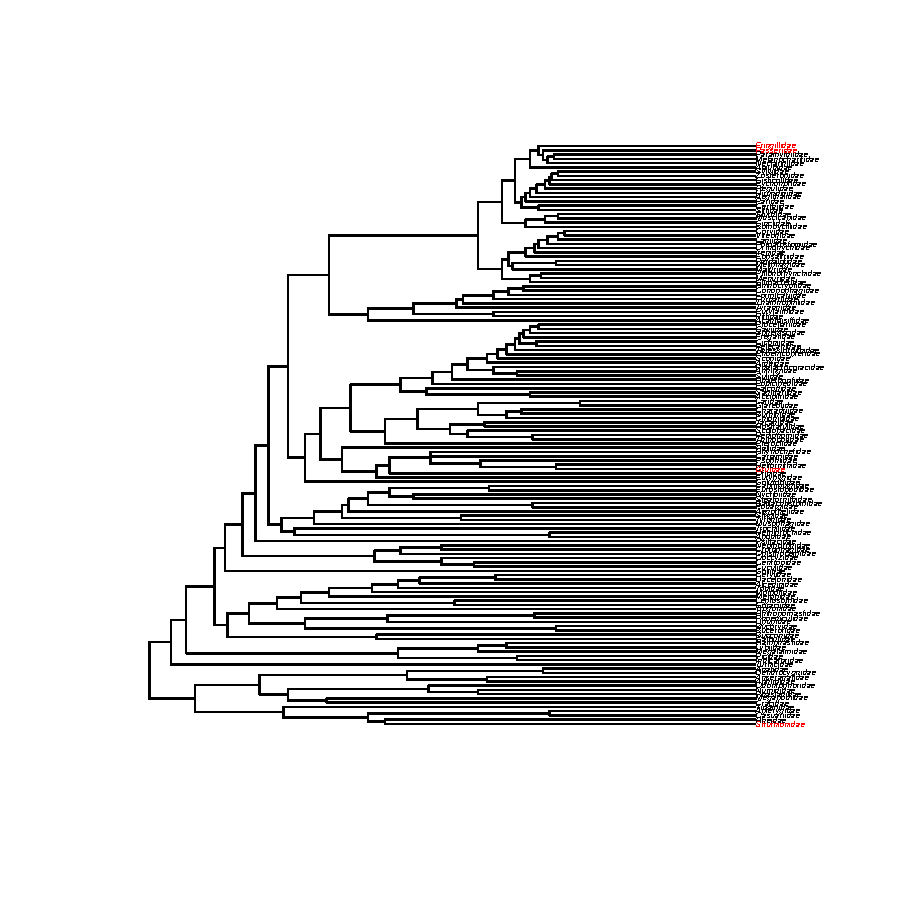
\includegraphics{Lecture6-005}
\end{center}
\caption{A phylogeny of bird families from \citet{Sibley.1990} The families in red are the \emph{Struthionidae} (Ostriches), \emph{Gruidae} (Cranes),  \emph{Passeridae} (Sparrows)  and \emph{Fringillidae} (Finches) from bottom to top.}
\label{bird.families-fig}
\end{figure}

\ifalone
\end{document}
\else
\fi

